\documentclass[12pt, english, oneside, open=any]{report}%draft
%---------------------------------------
%Language, text and grammer
\usepackage[utf8]{inputenc}
%Quotation marks
\usepackage{csquotes}
%Uk english text 
\usepackage{babel}

%Bibliography
\usepackage[square,comma,numbers]{natbib}
%List of accronyms, Nomenclature
\usepackage{longtable}
\usepackage[section,acronym]{glossaries}

\newacronym{ths}{THS}{ Thermal-hydraulic simulation}
\newacronym{plc}{PLC}{ Programmable logic controller}
\newacronym{scada}{SCADA}{ Supervisory control and data acquisition}
\newacronym{calds}{CALDS}{ Compressed Air Leakage Documentation System}
\newacronym{stb}{STB}{ Simulation Toolbox }
\newglossaryentry{kpa}{
	name = kPa ,
	description =  - Kilopascal
}
\newglossaryentry{mw}{
	name = MW ,
	description =  - MegaWatt
}

\newglossaryentry{t}{
	name = T,
	description =  - Tonne
}

\makeglossaries
%---------------------------------------

%APPEARANCE%
%% Page dimensions 
\usepackage{geometry}
\geometry{
	a4paper,
	left=25mm,
	right=20mm,
	top=20mm,
	bottom=25mm,
	headheight=110pt,
	heightrounded,
}

%%Chapter formatting 
\usepackage{titlesec}
\titleformat{\chapter}[display]
{\bfseries\Large}
{\filright\MakeUppercase{\chaptertitlename} \Huge\thechapter}
{0.5ex}
{\titlerule\filleft}
\usepackage{array}
\usepackage{calc}

%Set Spacing
\usepackage{setspace} 
\usepackage[hang, perpage]{footmisc}
\usepackage{lipsum}
\linespread{1.4}
\setlength{\parindent}{0em}
\setlength{\parskip}{1.5em}
\setlength{\belowcaptionskip}{-6pt} %set figure distance
\setlength{\skip\footins}{20pt}
\titlespacing*{\chapter}{0pt}{-38pt}{40pt}
\titlespacing*{\section}{0pt}{-10pt}{-15pt}
\titlespacing*{\subsection}{0pt}{-10pt}{-10pt}
\titlespacing*{\subsubsection}{0pt}{-10pt}{-10pt}
\titlespacing*{\paragraph}{0pt}{-10pt}{-10pt}
\usepackage{enumitem}
\setlist[itemize]{noitemsep, topsep=-10pt}
\setlist[enumerate]{noitemsep, topsep=-10pt}
\setlength{\glsdescwidth}{0.7\textwidth}
\setlength{\glspagelistwidth}{0.3\linewidth}
\usepackage{tocloft}
\setlength{\cftbeforesecskip}{3pt}
\setlength{\cftbeforechapskip}{6pt}
\setlength{\footnotemargin}{10pt}
\setlength{\footnotesep}{10pt}
\renewcommand\footnoterule{\rule{\textwidth}{1pt}}
\renewcommand{\arraystretch}{1.4}
%Page headers
\usepackage{fancyhdr}
\pagestyle{fancy}
\fancyhf{}
\renewcommand{\headrulewidth}{0.4pt}
\renewcommand{\footrulewidth}{0.3pt}
\rhead{\nouppercase{\leftmark}}
%\rhead{\rightmark}
\rfoot{\thepage}
\lfoot{\emph{ \color{black} Simulating operational improvements on mine compressed air systems}}
\makeatletter

%Links
\usepackage[hidelinks]{hyperref}
\usepackage{cleveref}


%Graphs 
\usepackage{graphics}
\usepackage{epstopdf}
\usepackage{color}
\usepackage[pdftex]{graphicx}
\usepackage{hhline}

%Title page
\usepackage[pages=some]{background}

\backgroundsetup
{
	scale=1,
	opacity=1,
	angle=0,
	contents={%
		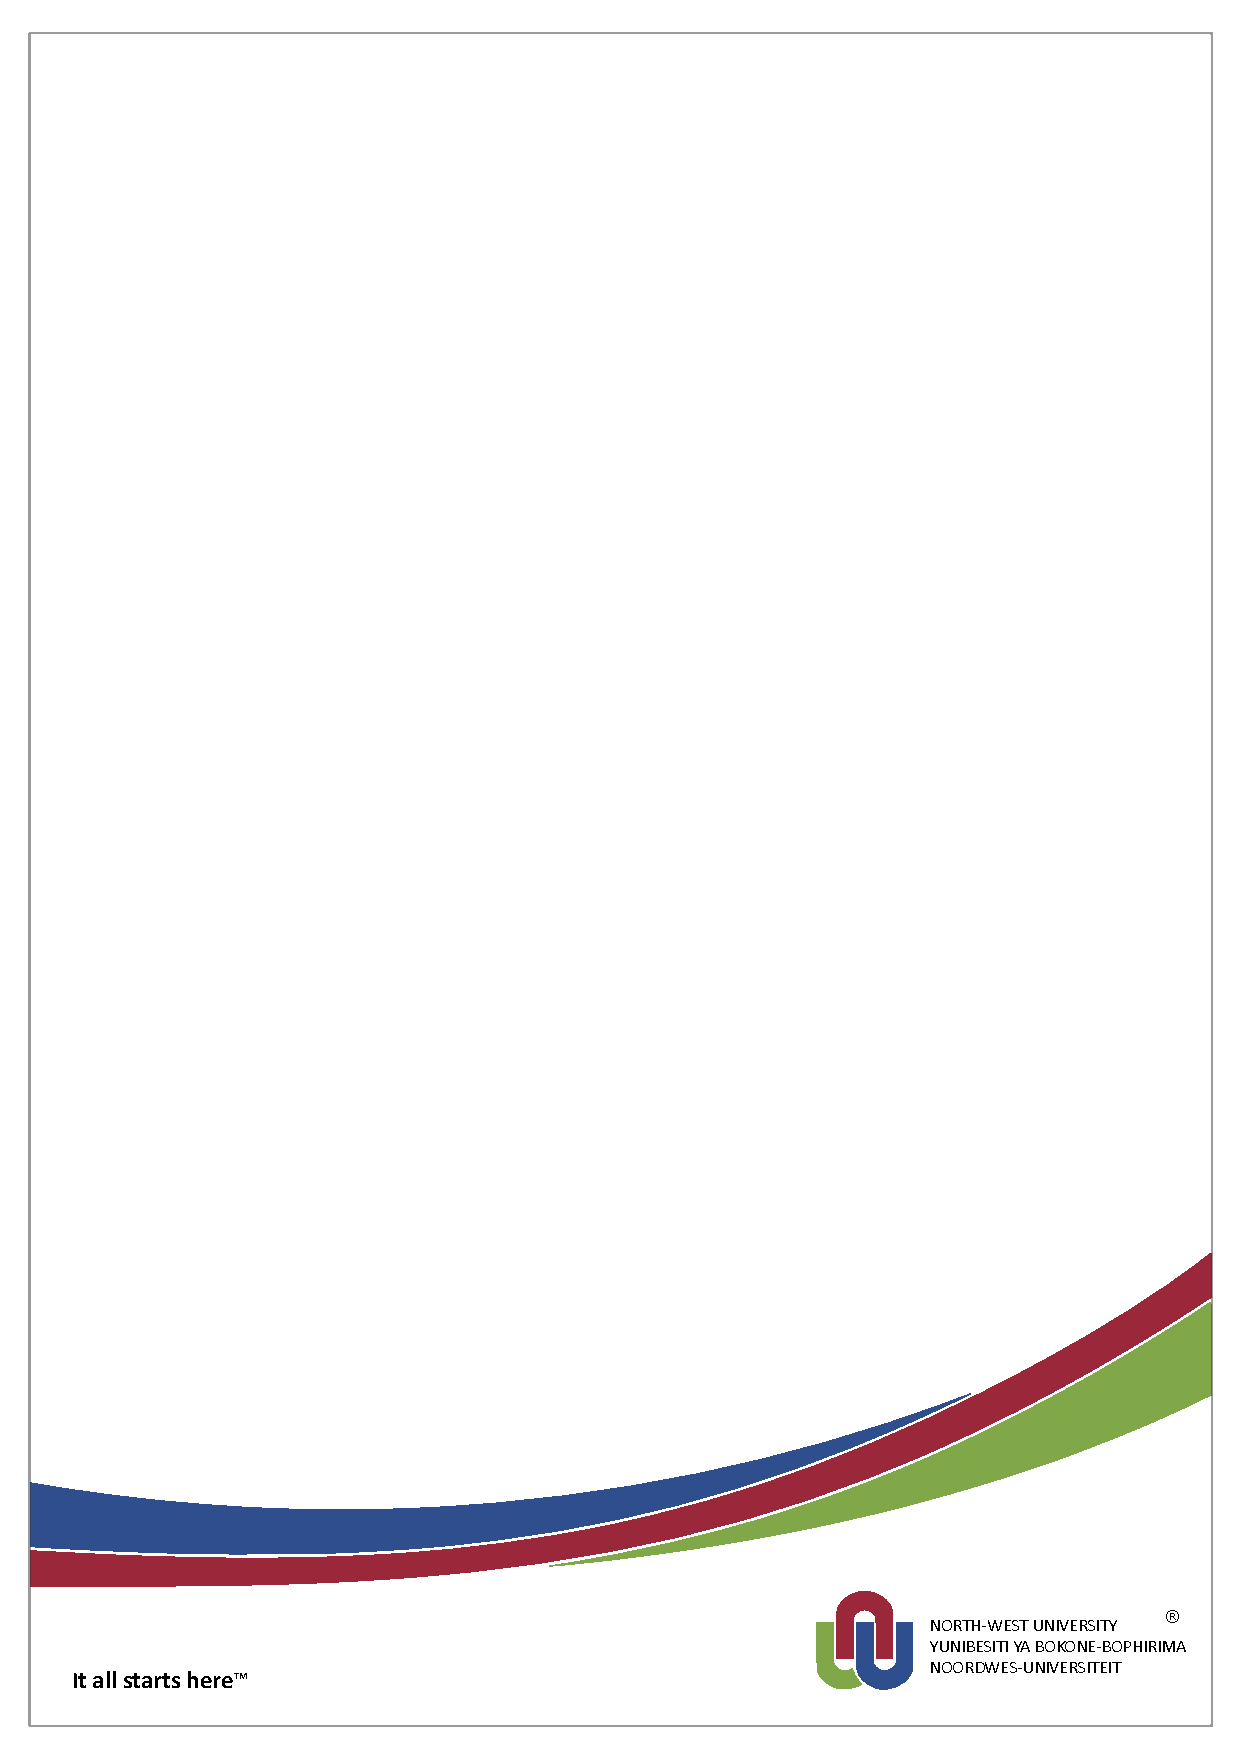
\includegraphics[width=\paperwidth,height=\paperheight]{Images/frontpage.pdf}
	}%
}
\usepackage{datetime}
\newdateformat{monthyeardate}{%
	\monthname[\THEMONTH], \THEYEAR}

%Table of contents page
\addtocontents{toc}{\protect\setcounter{tocdepth}{1}}
\usepackage[titletoc]{appendix}


\usepackage[ protrusion=true, expansion=true, final, babel ]{microtype}
%disable Ligatures (for word ocr conversion)
%\DisableLigatures{encoding = *, family = * }

 
 % Colors
 \definecolor{MasterBlue}{rgb}{0.18,0.45,0.71}


\begin{document}
\urlstyle{same}
\pagenumbering{roman}	
% Title page
\begin{titlepage}
	\BgThispage	
		\vspace{0cm}
		\begin{center}
			\textbf{\singlespacing\huge{Simulating operational improvements on mine compressed air systems}\\
			}\par
			\vspace{3cm}
			\LARGE{ \textbf{BM Friedenstein \\28354516} }
		\end{center}
	
	\vspace{2cm}
	
\begin{flushleft}
	{\singlespacing\centering \large Dissertation submitted in fulfilment of the requirements for the \\ degree {\color{MasterBlue} \textit{Master of Engineering}} in {\color{MasterBlue}Electrical and Electronic \\ Engineering} at the Potchefstroom Campus of the North-West\\ University\\
	}
	\vspace{2cm}
	{\large \setlength{\parindent}{0.5cm} Supervisor: Dr Johann van Rensburg \\
	\vspace{1cm}
	\large{Examination October 2017}\\		
	}
\end{flushleft}
\end{titlepage}
\clearpage

%Abstract
{\tiny }\section*{Abstract}
	\thispagestyle{plain}
	\vspace{0.2cm}
	\addcontentsline{toc}{chapter}{Abstract}
	\begin{tabular}{p{2.35cm}p{13cm}}
		\textbf{Title:} & Simulating operational improvements on mine compressed air systems  \\
		\textbf{Author:} & B.M. Friedenstein \\
		\textbf{Supervisor:} & Dr Johann van Rensburg \\
		\textbf{School:} & North-West University Potchefstroom Campus\\
		\textbf{Degree:} & Masters in Electrical and Electronic Engineering \\
	\end{tabular}
	\vspace{1cm}

As operational costs of deep level mines increase, and gold ore grades decrease, profitability in the South African gold mining sector is becoming a challenge. Electricity tariff increases have contributed to this rise in the cost of operating mines.

	 \par
Compressed air supply systems are the largest energy users in a mine, contributing to approximately 20\% of their total power usage. It has been shown that mining compressed air networks are systemically inefficient. Improving the efficiency of these systems would result in a reduction of energy costs.
	 \par
Previous studies have shown the usefulness of simulations to develop improvements for deep level mining systems. However, these studies have not followed a structured methodology for developing compressed air simulations. Previous studies also used simplified compressed air models, therefore, reducing the simulation precision and testable scenarios.

	\par
In this study, a simulation methodology was developed. Investigations into the compressed air systems are also performed. A compressed air system is then modelled in adequate software to recreate the system operation accurately. Finally, a proposed means of improvement is simulated, analysed and quantified regarding improvements in energy savings and service delivery.
	 \par
Two case studies were evaluated. For each case study, a variety of scenarios were simulated. In Case study 1, two scenarios were simulated on a compressed air system. The results showed that energy cost savings of R0.91M could be achieved. The simulation results were very similar to tests later performed on the physical systems.
	 \par 
The results of case study 2 showed that by reducing air usage at refuge bays, an average power reduction of 1 MW could be achieved. The improvement in efficiency would potentially lead to R 5.2m in annual energy cost savings. Additionally, a significant improvement of 15 kPa to system pressure during the drilling period were identified. Other scenarios showed annual energy cost savings of up to R 2.5m.
	 \par 
An additional analysis was implemented to assess the use of periodically repeated simulations. The results demonstrated that through repeated simulations, operational changes in a system could continuously be identified. This information can then be used for further improvement and cost savings.
	 \par
The study showed that a simulation is a valuable tool for the identification of improvements in compressed air systems. By utilising a structured methodology to develop detailed compressed air simulations, inefficiencies and operational improvements were successfully identified.
	 \par
	\begin{tabular}{p{2.35cm}p{13.35cm}}
		\textbf{Keywords:} & Simulation,  compressed air, energy, mining, operational improvements  \\
	\end{tabular}
\clearpage

{\tiny }\section*{Acknowledgements}
\thispagestyle{plain}
\vspace{0.2cm}
\addcontentsline{toc}{chapter}{Acknowledgements}
\clearpage

\tableofcontents

\clearpage

\renewcommand{\arraystretch}{1.2}
\linespread{1}
%List of symbals
%List of abreviations
	\addcontentsline{toc}{chapter}{Abbreviations and nomenclature}
	\printglossary[type=\acronymtype]
	\newpage
	\printglossary[title=Nomenclature]
	\newpage
\renewcommand{\arraystretch}{1.4}
\linespread{1.4}

	%\printglossaries	
	\addcontentsline{toc}{chapter}{List of figures and tables}
	\listoffigures
	\clearpage
	\listoftables

%Chapters
%Chapter 1
\chapter{Introduction and background}  %J.H Marais, C.J.R. Kriel
\pagenumbering{arabic} 
\setcounter{page}{1}
\section{Preamble}

\section{Background on deep level mining}
\subsection{Mining profitability}
\subsection{Mining systems and energy usage}
\subsection{Need to reduce inefficiencies and improve service delivery}
\section{Mining compressed air systems}
	\subsection{Characteristic inefficiencies}
	\subsection{Inefficiency identification methods}
	\subsection{Instrumentation and measurements}
\section{Use of simulation in industry}
\section{Problem statement}
\section{Dissertation overview}
%Chapter 2
\chapter{Overview of simulation and compressed air applications}
\thispagestyle{empty}
\vspace{38em}
\hrulefill
\\
\enquote*{\textit{Quote.}} - Somebody\\
\clearpage
\section{Introduction}
\section{Review of compressed air energy interventions in industry}
	\subsection{Preamble}
		Compressed air improvement can be obtained through intervention in either the supply or demand of compressed air \cite{Kriel2014Masters}. Improvements in supply interventions are achieved by increasing the efficiency of compressed air supply. Examples of this type of intervention include \gls{dcs}, compressor maintenance, etc. 
		\par
		Due to the size of mining compressed air networks, there is often a larger scope for improvement in air demand. Improving the  demand is achieved by optimising air flow consumers, reducing leaks, etc.
		\par
	 	From literature, this section will review compressed air energy interventions that have performed in industry.
	 	
	\subsection{Strategies to improve compressed air supply}
	
		\subsubsection{Optimising compressor control}
		Compressors types and numbers can differ widely from mining compressed air systems. Compressor selection is crucial in these systems to match the correct compressors with the requirements of the system \cite{marais2010expert}.
		\par 
		In a study by Booysen \textit{et al} \cite{Booysen2012Masters} on optimising compressor control, \cite{Booysen2012Masters} found that many mines control compressors using fixed target pressure points that are much higher that required. In one system, compressors were set to a target 650 \gls{kpa} to ensure pressure underground did not fall below 500 \gls{kpa}. Using high pressure set-points can lead to excessive wasteful blow-off flow when the pressure exceeds a maximum points.
		\par 
		Booysen \cite{booysen2009optimising} showed that through dynamic pressure setpoint control, matching the supply pressure with the demand, and optimal compressor selection, energy savings can be achieved. In a case study, an average power reduction of 1.07 MW was achieved. The lead to an estimated energy cost saving of R3M.
		
		\par 
		- Variable speed drives\\
		
		\subsection{Air storage}
		- booysen 1.22
		\subsubsection{Dynamic compressor selection}
		
		\subsubsection{Reconfiguring compressed air networks}
			A number of old mining compressed air systems  have not been adequately maintained and improved. Often they cannot sufficiently supply air to meet the demand or air is provided from non optimal sources. In a study by Bredenkamp \cite{Bredenkamp2013Masters}, reconfiguring of the air network was investigated to improve these systems.
			\par  
			In the study, Bredenkamp investigated interconnecting the compressed air systems of two mining shafts and relocating of a compressor. This strategy lead to an average power reduction of 1.7 MW and an estimated annual energy cost saving of R8.9M at the time.
			\par 
			\textit{Discussion of Bredenkamp}
			
	\subsection{Strategies to reduce compressed air demand}
	As illustrated in \cref{fig: Mining schedule}
		- Reducing leaks\\
		- 
		- Marais PhD\\
		- Snyman - investigated various Compressed air demand reduction and efficiency
		 optimisations \cite{Snyman2011Masters}.
		 
		 \subsubsection{Leakage detection}
		 Air leaks are a major inefficiency in mining compressed air systems. Improving leaks is relatively easier method to  reduce air demand and improve the efficiency of the system  \cite{van2011sustaining}. Air leaks occur as a result of open pipes, fissure and breaks. Losses depend on the size of the leak. \cref{fig: Leak losses} shows the estimated power losses vs leakage area.
		 \par
		 ***Fix this  booysen 1.20 ***
		 \begin{figure}[h]
		 	\centering
		 	% GNUPLOT: LaTeX picture with Postscript
\begingroup
  \makeatletter
  \providecommand\color[2][]{%
    \GenericError{(gnuplot) \space\space\space\@spaces}{%
      Package color not loaded in conjunction with
      terminal option `colourtext'%
    }{See the gnuplot documentation for explanation.%
    }{Either use 'blacktext' in gnuplot or load the package
      color.sty in LaTeX.}%
    \renewcommand\color[2][]{}%
  }%
  \providecommand\includegraphics[2][]{%
    \GenericError{(gnuplot) \space\space\space\@spaces}{%
      Package graphicx or graphics not loaded%
    }{See the gnuplot documentation for explanation.%
    }{The gnuplot epslatex terminal needs graphicx.sty or graphics.sty.}%
    \renewcommand\includegraphics[2][]{}%
  }%
  \providecommand\rotatebox[2]{#2}%
  \@ifundefined{ifGPcolor}{%
    \newif\ifGPcolor
    \GPcolortrue
  }{}%
  \@ifundefined{ifGPblacktext}{%
    \newif\ifGPblacktext
    \GPblacktextfalse
  }{}%
  % define a \g@addto@macro without @ in the name:
  \let\gplgaddtomacro\g@addto@macro
  % define empty templates for all commands taking text:
  \gdef\gplbacktext{}%
  \gdef\gplfronttext{}%
  \makeatother
  \ifGPblacktext
    % no textcolor at all
    \def\colorrgb#1{}%
    \def\colorgray#1{}%
  \else
    % gray or color?
    \ifGPcolor
      \def\colorrgb#1{\color[rgb]{#1}}%
      \def\colorgray#1{\color[gray]{#1}}%
      \expandafter\def\csname LTw\endcsname{\color{white}}%
      \expandafter\def\csname LTb\endcsname{\color{black}}%
      \expandafter\def\csname LTa\endcsname{\color{black}}%
      \expandafter\def\csname LT0\endcsname{\color[rgb]{1,0,0}}%
      \expandafter\def\csname LT1\endcsname{\color[rgb]{0,1,0}}%
      \expandafter\def\csname LT2\endcsname{\color[rgb]{0,0,1}}%
      \expandafter\def\csname LT3\endcsname{\color[rgb]{1,0,1}}%
      \expandafter\def\csname LT4\endcsname{\color[rgb]{0,1,1}}%
      \expandafter\def\csname LT5\endcsname{\color[rgb]{1,1,0}}%
      \expandafter\def\csname LT6\endcsname{\color[rgb]{0,0,0}}%
      \expandafter\def\csname LT7\endcsname{\color[rgb]{1,0.3,0}}%
      \expandafter\def\csname LT8\endcsname{\color[rgb]{0.5,0.5,0.5}}%
    \else
      % gray
      \def\colorrgb#1{\color{black}}%
      \def\colorgray#1{\color[gray]{#1}}%
      \expandafter\def\csname LTw\endcsname{\color{white}}%
      \expandafter\def\csname LTb\endcsname{\color{black}}%
      \expandafter\def\csname LTa\endcsname{\color{black}}%
      \expandafter\def\csname LT0\endcsname{\color{black}}%
      \expandafter\def\csname LT1\endcsname{\color{black}}%
      \expandafter\def\csname LT2\endcsname{\color{black}}%
      \expandafter\def\csname LT3\endcsname{\color{black}}%
      \expandafter\def\csname LT4\endcsname{\color{black}}%
      \expandafter\def\csname LT5\endcsname{\color{black}}%
      \expandafter\def\csname LT6\endcsname{\color{black}}%
      \expandafter\def\csname LT7\endcsname{\color{black}}%
      \expandafter\def\csname LT8\endcsname{\color{black}}%
    \fi
  \fi
    \setlength{\unitlength}{0.0500bp}%
    \ifx\gptboxheight\undefined%
      \newlength{\gptboxheight}%
      \newlength{\gptboxwidth}%
      \newsavebox{\gptboxtext}%
    \fi%
    \setlength{\fboxrule}{0.5pt}%
    \setlength{\fboxsep}{1pt}%
\begin{picture}(9360.00,4032.00)%
    \gplgaddtomacro\gplbacktext{%
      \colorrgb{0.00,0.00,0.00}%
      \put(946,704){\makebox(0,0)[r]{\strut{}$0$}}%
      \colorrgb{0.00,0.00,0.00}%
      \put(946,1087){\makebox(0,0)[r]{\strut{}$1000$}}%
      \colorrgb{0.00,0.00,0.00}%
      \put(946,1470){\makebox(0,0)[r]{\strut{}$2000$}}%
      \colorrgb{0.00,0.00,0.00}%
      \put(946,1853){\makebox(0,0)[r]{\strut{}$3000$}}%
      \colorrgb{0.00,0.00,0.00}%
      \put(946,2236){\makebox(0,0)[r]{\strut{}$4000$}}%
      \colorrgb{0.00,0.00,0.00}%
      \put(946,2618){\makebox(0,0)[r]{\strut{}$5000$}}%
      \colorrgb{0.00,0.00,0.00}%
      \put(946,3001){\makebox(0,0)[r]{\strut{}$6000$}}%
      \colorrgb{0.00,0.00,0.00}%
      \put(946,3384){\makebox(0,0)[r]{\strut{}$7000$}}%
      \colorrgb{0.00,0.00,0.00}%
      \put(946,3767){\makebox(0,0)[r]{\strut{}$8000$}}%
      \colorrgb{0.00,0.00,0.00}%
      \put(1078,484){\makebox(0,0){\strut{}$0$}}%
      \colorrgb{0.00,0.00,0.00}%
      \put(2310,484){\makebox(0,0){\strut{}$5000$}}%
      \colorrgb{0.00,0.00,0.00}%
      \put(3542,484){\makebox(0,0){\strut{}$10000$}}%
      \colorrgb{0.00,0.00,0.00}%
      \put(4774,484){\makebox(0,0){\strut{}$15000$}}%
      \colorrgb{0.00,0.00,0.00}%
      \put(6006,484){\makebox(0,0){\strut{}$20000$}}%
      \colorrgb{0.00,0.00,0.00}%
      \put(7237,484){\makebox(0,0){\strut{}$25000$}}%
      \colorrgb{0.00,0.00,0.00}%
      \put(8469,484){\makebox(0,0){\strut{}$30000$}}%
    }%
    \gplgaddtomacro\gplfronttext{%
      \csname LTb\endcsname%
      \put(176,2235){\rotatebox{-270}{\makebox(0,0){\strut{}Power loss (kW)}}}%
      \put(5020,154){\makebox(0,0){\strut{}Leak size ($mm^2$)}}%
    }%
    \gplbacktext
    \put(0,0){\fbox{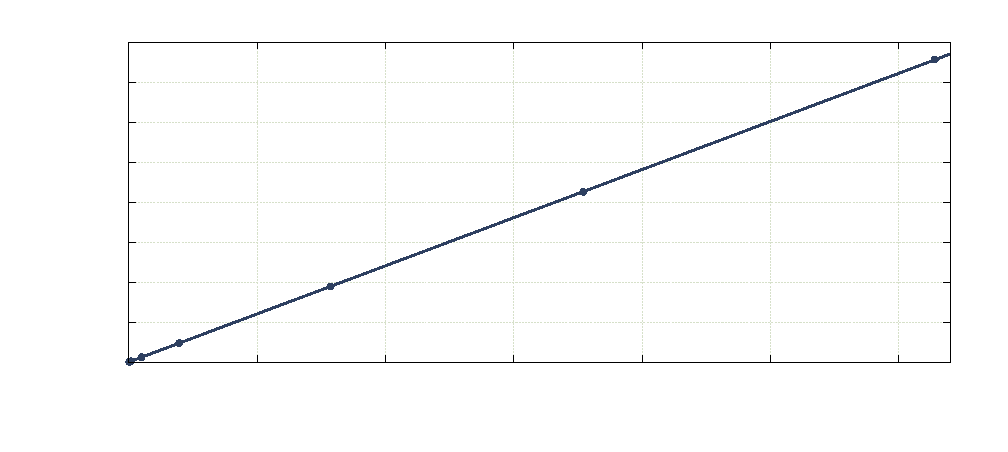
\includegraphics[trim=0 0 0.1cm 0, clip]{Graphs/2/Leak/Leak}}}%
    \gplfronttext
  \end{picture}%
\endgroup

		 	\caption[The estimated power loss vs leakage area.]{ The estimated power loss vs leakage area \cite{van2011sustaining}.}
		 	\label{fig: Leak losses}
		 \end{figure}
		 Air is often not easily detected through visual methods. In industry, a number of techniques are employed to detect air leaks. Pascoe \cite{Pascoe2016Masters} and van Tonder \cite{vanTonder2010Masters} summarised these strategies as follows:
		 \begin{itemize}
		 	\item Audible detection (Walk and report)
		 	\item Ultrasonic detection
		 	\item Detection through intelligent systems
		 	\item Pigging
		 	\item soap water and dyes
		 \end{itemize}
	 	 These methods can be time and resource intensive and many mines do not actively employ dedicated leakage detection repair teams. Marais \textit{et al} \cite{marais2009increased} investigated streamlining the leakage detection and repair process to increase energy savings through the use of \gls{calds}. The \gls{calds} system was developed to allow centralised mobile leakage reporting. Usage of the system resulted in increased leak detection rate with one mine reporting 24 leaks in a single month. It was noted in the study that there difficulty quantifying the actual energy savings of the leakage repairs due to other intervention occurring simultaneously.	
		 
		 \subsubsection{Underground control valves}
		 - Pascoe
		 
		\subsubsection{Improving pneumatic rock drills efficiency}
		 Pneumatic rock drills are on of the largest air consumers in a mine. Improving the efficiency or drilling can have a significant energy impact of the system. In a study by  Bester \textit{et al.} \cite{bester2013effect} looking at the effect of compressed air pressure on energy demand. Bester showed that between 2002 and 2013 compressed air and energy consumption per tonne of ore produced had steadily increased. This is illustrated  in \cref{fig: Compressed energy and air flow per ton}. 
		 \par 
		 The increase of air consumption per \gls{t} was a result of reduced air pressure at the mining areas. This causes the drilling rate to drop leading to higher air consumption. Pressure measurements as low as 300 \gls{kpa} were recorded in these areas. Before 2002 the drilling pressure at the mining section (stopes), was maintained above 500 \gls{kpa} at most mines. 
		 \par 
		 \begin{figure}[h]
		 	\centering
		 	% GNUPLOT: LaTeX picture with Postscript
\begingroup
  \makeatletter
  \providecommand\color[2][]{%
    \GenericError{(gnuplot) \space\space\space\@spaces}{%
      Package color not loaded in conjunction with
      terminal option `colourtext'%
    }{See the gnuplot documentation for explanation.%
    }{Either use 'blacktext' in gnuplot or load the package
      color.sty in LaTeX.}%
    \renewcommand\color[2][]{}%
  }%
  \providecommand\includegraphics[2][]{%
    \GenericError{(gnuplot) \space\space\space\@spaces}{%
      Package graphicx or graphics not loaded%
    }{See the gnuplot documentation for explanation.%
    }{The gnuplot epslatex terminal needs graphicx.sty or graphics.sty.}%
    \renewcommand\includegraphics[2][]{}%
  }%
  \providecommand\rotatebox[2]{#2}%
  \@ifundefined{ifGPcolor}{%
    \newif\ifGPcolor
    \GPcolortrue
  }{}%
  \@ifundefined{ifGPblacktext}{%
    \newif\ifGPblacktext
    \GPblacktextfalse
  }{}%
  % define a \g@addto@macro without @ in the name:
  \let\gplgaddtomacro\g@addto@macro
  % define empty templates for all commands taking text:
  \gdef\gplbacktext{}%
  \gdef\gplfronttext{}%
  \makeatother
  \ifGPblacktext
    % no textcolor at all
    \def\colorrgb#1{}%
    \def\colorgray#1{}%
  \else
    % gray or color?
    \ifGPcolor
      \def\colorrgb#1{\color[rgb]{#1}}%
      \def\colorgray#1{\color[gray]{#1}}%
      \expandafter\def\csname LTw\endcsname{\color{white}}%
      \expandafter\def\csname LTb\endcsname{\color{black}}%
      \expandafter\def\csname LTa\endcsname{\color{black}}%
      \expandafter\def\csname LT0\endcsname{\color[rgb]{1,0,0}}%
      \expandafter\def\csname LT1\endcsname{\color[rgb]{0,1,0}}%
      \expandafter\def\csname LT2\endcsname{\color[rgb]{0,0,1}}%
      \expandafter\def\csname LT3\endcsname{\color[rgb]{1,0,1}}%
      \expandafter\def\csname LT4\endcsname{\color[rgb]{0,1,1}}%
      \expandafter\def\csname LT5\endcsname{\color[rgb]{1,1,0}}%
      \expandafter\def\csname LT6\endcsname{\color[rgb]{0,0,0}}%
      \expandafter\def\csname LT7\endcsname{\color[rgb]{1,0.3,0}}%
      \expandafter\def\csname LT8\endcsname{\color[rgb]{0.5,0.5,0.5}}%
    \else
      % gray
      \def\colorrgb#1{\color{black}}%
      \def\colorgray#1{\color[gray]{#1}}%
      \expandafter\def\csname LTw\endcsname{\color{white}}%
      \expandafter\def\csname LTb\endcsname{\color{black}}%
      \expandafter\def\csname LTa\endcsname{\color{black}}%
      \expandafter\def\csname LT0\endcsname{\color{black}}%
      \expandafter\def\csname LT1\endcsname{\color{black}}%
      \expandafter\def\csname LT2\endcsname{\color{black}}%
      \expandafter\def\csname LT3\endcsname{\color{black}}%
      \expandafter\def\csname LT4\endcsname{\color{black}}%
      \expandafter\def\csname LT5\endcsname{\color{black}}%
      \expandafter\def\csname LT6\endcsname{\color{black}}%
      \expandafter\def\csname LT7\endcsname{\color{black}}%
      \expandafter\def\csname LT8\endcsname{\color{black}}%
    \fi
  \fi
    \setlength{\unitlength}{0.0500bp}%
    \ifx\gptboxheight\undefined%
      \newlength{\gptboxheight}%
      \newlength{\gptboxwidth}%
      \newsavebox{\gptboxtext}%
    \fi%
    \setlength{\fboxrule}{0.5pt}%
    \setlength{\fboxsep}{1pt}%
\begin{picture}(9360.00,4032.00)%
    \gplgaddtomacro\gplbacktext{%
      \colorrgb{0.42,0.42,0.42}%
      \put(682,924){\makebox(0,0)[r]{\strut{}$0$}}%
      \colorrgb{0.42,0.42,0.42}%
      \put(682,1230){\makebox(0,0)[r]{\strut{}$5$}}%
      \colorrgb{0.42,0.42,0.42}%
      \put(682,1536){\makebox(0,0)[r]{\strut{}$10$}}%
      \colorrgb{0.42,0.42,0.42}%
      \put(682,1842){\makebox(0,0)[r]{\strut{}$15$}}%
      \colorrgb{0.42,0.42,0.42}%
      \put(682,2148){\makebox(0,0)[r]{\strut{}$20$}}%
      \colorrgb{0.42,0.42,0.42}%
      \put(682,2453){\makebox(0,0)[r]{\strut{}$25$}}%
      \colorrgb{0.42,0.42,0.42}%
      \put(682,2759){\makebox(0,0)[r]{\strut{}$30$}}%
      \colorrgb{0.42,0.42,0.42}%
      \put(682,3065){\makebox(0,0)[r]{\strut{}$35$}}%
      \colorrgb{0.42,0.42,0.42}%
      \put(682,3371){\makebox(0,0)[r]{\strut{}$40$}}%
      \colorrgb{0.42,0.42,0.42}%
      \put(814,704){\makebox(0,0){\strut{}$2002$}}%
      \colorrgb{0.42,0.42,0.42}%
      \put(2025,704){\makebox(0,0){\strut{}$2004$}}%
      \colorrgb{0.42,0.42,0.42}%
      \put(3237,704){\makebox(0,0){\strut{}$2006$}}%
      \colorrgb{0.42,0.42,0.42}%
      \put(4448,704){\makebox(0,0){\strut{}$2008$}}%
      \colorrgb{0.42,0.42,0.42}%
      \put(5659,704){\makebox(0,0){\strut{}$2010$}}%
      \colorrgb{0.42,0.42,0.42}%
      \put(6871,704){\makebox(0,0){\strut{}$2012$}}%
      \colorrgb{0.42,0.42,0.42}%
      \put(8082,704){\makebox(0,0){\strut{}$2014$}}%
      \colorrgb{0.42,0.42,0.42}%
      \put(8214,924){\makebox(0,0)[l]{\strut{}$0$}}%
      \colorrgb{0.42,0.42,0.42}%
      \put(8214,1230){\makebox(0,0)[l]{\strut{}$50$}}%
      \colorrgb{0.42,0.42,0.42}%
      \put(8214,1536){\makebox(0,0)[l]{\strut{}$100$}}%
      \colorrgb{0.42,0.42,0.42}%
      \put(8214,1842){\makebox(0,0)[l]{\strut{}$150$}}%
      \colorrgb{0.42,0.42,0.42}%
      \put(8214,2148){\makebox(0,0)[l]{\strut{}$200$}}%
      \colorrgb{0.42,0.42,0.42}%
      \put(8214,2453){\makebox(0,0)[l]{\strut{}$250$}}%
      \colorrgb{0.42,0.42,0.42}%
      \put(8214,2759){\makebox(0,0)[l]{\strut{}$300$}}%
      \colorrgb{0.42,0.42,0.42}%
      \put(8214,3065){\makebox(0,0)[l]{\strut{}$350$}}%
      \colorrgb{0.42,0.42,0.42}%
      \put(8214,3371){\makebox(0,0)[l]{\strut{}$400$}}%
    }%
    \gplgaddtomacro\gplfronttext{%
      \csname LTb\endcsname%
      \put(176,2147){\rotatebox{-270}{\makebox(0,0){\strut{}kWh/t}}}%
      \put(8851,2147){\rotatebox{-270}{\makebox(0,0){\strut{}$m^3$/t}}}%
      \put(4448,374){\makebox(0,0){\strut{}Year}}%
      \put(4448,3701){\makebox(0,0){\strut{}Compressed air energy and Volume consumed per ton}}%
      \csname LTb\endcsname%
      \put(3593,173){\makebox(0,0)[r]{\strut{}Energy per Ton (kWh/t)}}%
      \csname LTb\endcsname%
      \put(7352,173){\makebox(0,0)[r]{\strut{}Volume per Ton ($m^3$/t)}}%
    }%
    \gplbacktext
    \put(0,0){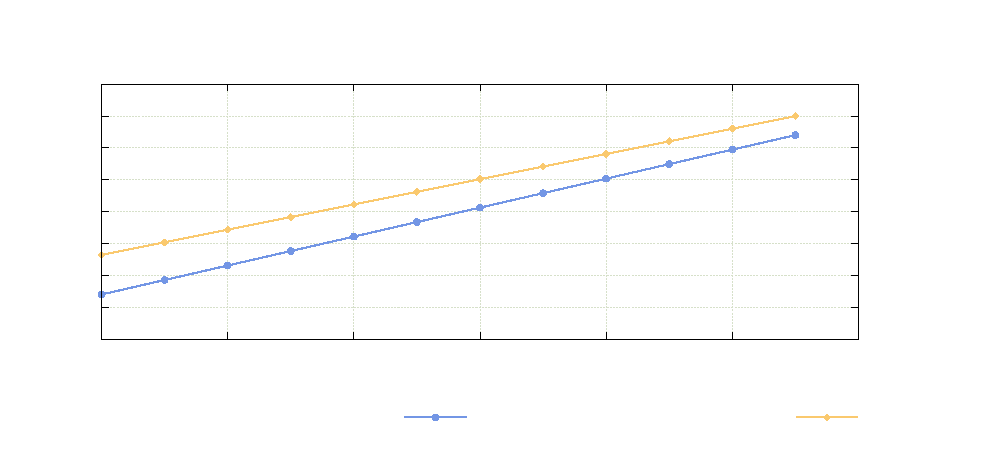
\includegraphics{Graphs/1/EVperT/EVperT}}%
    \gplfronttext
  \end{picture}%
\endgroup

		 	\caption[The Compressed air energy and flow consumed per T of ore produced.]{The Compressed air energy and flow consumed per T of ore produced. Adopted from Bester \textit{et al.} \cite{bester2013effect}.}
		 	\label{fig: Compressed energy and air flow per ton}
		 \end{figure}
		 From the literature, it is shown that lowering the pressure reduces the efficiency and drill rate of rock drilling, leading to higher air consumption. Interventions that reduce systemic air losses or optimise supply can increase the pressure operating pressure. Increased pressure, during the drilling shift, may add more value than the energy cost savings that can be achieved at a lower pressure.
	\subsection{Summary}
\clearpage

\section{Use of simulations to identify improvements in mining systems}
	\subsection{Preamble}
	\subsection{Simulation tools}
	\subsection{Value of simulation in DSM projects}
		(Van Niekerk M)\\
		- Compressed air \\
		- Cooling systems\\
		- Dewatering\\
		- Design optimisations using simulation\\
		- De Coning -  simulations to investigate the opportunity to optimise the control strategy of a compressed air network by rescheduling the compressors.
	\subsection{Simulation procedures}
	
		-Kriel masters\\
		 \glspl{vsd} (or \glspl{vfd}) \\
		-Pascoe
		\subsubsection{Periodic simulation}
 	\subsection{Verifying simulations}
 		— Holman
 		— van Niekerk masters\\
 		— Kriel masters ( validation)\\
 		— Calibrating -pascoe\\
 		— determining accuracy - pascoe\\
 		— Du2015Development\\
 		— comparisons with models\\
 		— comparison with actual \\
 		— First principles\\
 	
	
	\section{Use of simulation in compressed air system optimisation}
	
	\subsection{Estimation techniques}
	- Snyman estimated improvements using historical data.\cite{Snyman2011Masters}\\
	- Marais estimation through simplified estimation, simulation \cite{Marais2012PhD, marais2013simplification}.
	\clearpage	
	
	\subsubsection{Shortcoming of previous studies}
		\label{Shortcomings of previous work}
	\subsection{Summary}
\section{Conclusion}
%Chapter 3
\chapter{Developing a simulation methodology}
\thispagestyle{empty}
\vspace{38em}
\hrulefill
\\
\enquote*{\textit{Great Design is iteration of good design.}} - Dr M. Cobanli\\
\newpage
\section{Introduction}
This chapter details the implementation methodology of simulations to optimize mining compressed air systems. The methodology discussed in this chapter will utilize insights from previous studies. Improving on shortcomings discussed in section \ref{Shortcomings of previous work}.
\par 
Implementation of a simulation is divided into three steps as shown in the flow diagram, Figure \ref{fig: Methodology}. Firstly, an investigation on the specific air network to is performed. The data acquired from this investigation is then utilized to develop and verify a simulation model. In the final step, scenarios are tested using simulations and the results are quantified and prioritised. After the process has been reviewed, a simulation  report is then produced and passed to the mine.
\begin{figure}[h]
	\centering
	\fbox{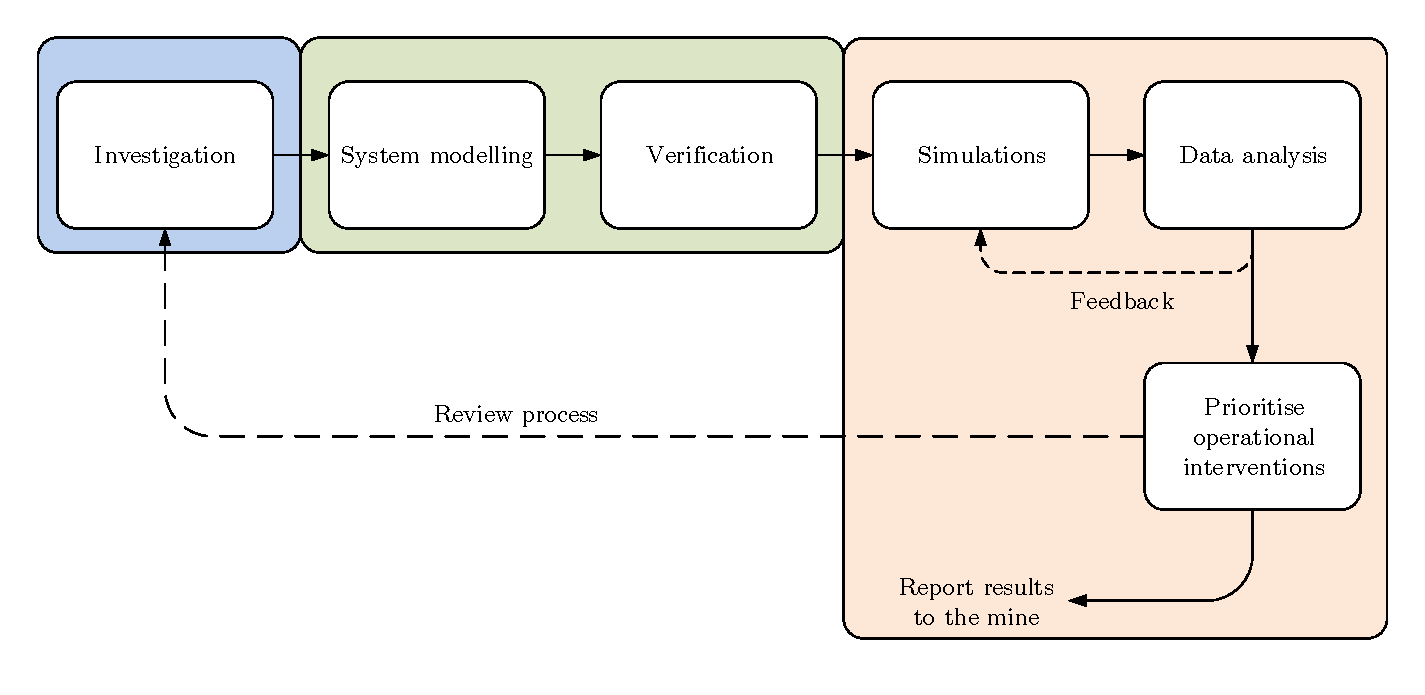
\includegraphics[trim=-0.5cm 0.8cm -0.5cm 0.5cm,width=\textwidth]{Graphs/3/Methodology/Methodology.pdf}}
	\caption{Flow diagram of the methodology for this study.}
	\label{fig: Methodology}
\end{figure}
\newpage
\section{System investigation method}
	\subsection{Preamble}
		Developing a detailed simulation model of a compressed air network requires thorough comprehension of the inner workings of the system. This section will discuss the investigations needed to obtain the required understanding.
	\subsection{Acquiring data} % 
	The first step of the system investigation is to acquire the data and understanding that will be required to model compressed air system's function. This will require access to mine resources such as data storage systems, instrumentation, and communication with relevant engineers and personnel.
	\par 
	Comprehensive and up to date layouts illustrate a compressed air network's unique set-up, scale and location of instrumentation. More detailed layouts can provide per-level air consumption breakdowns of the network, locations of refuge bays, mining cross-sections and identified inefficiencies. This is vital to understand the operation and identify what data parameters will be required for the model. 
	\par 
	A baseline period that best represents the typical operation of the mine. Additionally, availability of data should be considered. The length of the baseline period is selected based on the scenarios that are to be tested, this can be changed later. For calibrating a compressed air system a 24 hours period of normal operation is usually sufficient. A longer period may be needed to verify the model.
	Next data 
	\subsection{Mining schedule}
	A critical aspect to developing an accurate model of a mining compressed air system is apprehension of the operational philosophy of the mine. The schedule for operations such as drilling,  blasting or cleaning can have a major impact on compressed air requirements at different times of the day. By utilizing the operational schedule, simulation scenarios can be optimized for the air requirements throughout the day.	
	
	\subsection{Data verification}
	Data verification is the process where data is evaluated to ensure accuracy. It is important to verify data that is used for model development as an accurate representation of the operation of a system can only be achieved utilising data of high quality \cite{gous2016data}. The factors that influence a data-set's quality, accuracy and integrity  summarised as follows:
	\begin{itemize}
		\item Conversion of measurement value \cite{meijsen2015verification}
		\item Storage and collection of the system \cite{vanNiekerk2016quantification},\cite{Jansevan2016structuring}
		\item Traceability of measurement sources \cite{Jansevan2016structuring}
		\item Measurement equipment accuracy and malfunctions \cite{gous2016data}
		\item Data abnormalities \cite{gous2016data}
	\end{itemize} 
	\par 
	Therefore a data verification methodology is utilised to ensure datasets are of high quality. 
	\subsection{Solutions to unavailable data}
		Parameters that are required to develop the simulation model, such as flows, pressures, may not be actively logged by mine systems. To obtain this data it is necessary to investigate alternative sources. At points where instrumentation is absent, estimations can be made from assumptions made using instrumentation on the network or spot inspections.
		\par 
		Air network specifications such as piping sizes, technical layouts, major leak locations or specifications is often outdated or not recorded. Critical data should be obtained through audits and inspections of the system. If manual inspection is not possible, estimations should be made using the available data or approximation techniques discussed in literature. %\texttt{REMEMBER TO REFERENCE\\ SPECIFIC LOCATION LITERATURE}.
	
	\subsection{Summary}
\newpage	
\section{Model development and verification}
	\subsection{Preamble}
	Compressed air networks are comprised of components such as compressors, valves, pipes, etc. This section will discuss the development, calibration and verification of component models that make up a compressed air simulation. 
	\subsection{Compressed air component models}
		\subsubsection{Air pipes}
		Pressure losses occur over compressed air networks due to friction in the pipe, these losses should be taken into account in the simulation for large piping sections. A pipe model is used to account for these losses which are defined by the \textit{Darcy-Weisbach equation}\footnote{ B. Glenn, \enquote*{The Darcy–Weisbach Equation,}[Online] \url{https://bae.okstate.edu/faculty-sites/Darcy/DarcyWeisbach/Darcy-WeisbachEq.htm}, [Accessed 20-05-2017]}:
		$$\Delta P = \frac{f  L \rho V^2}{2 D}$$
		Where the pressure difference $\Delta P $ is a function of:\\
		\begin{tabular}{p{1.3cm}p{13cm}}
		$f$ & Friction coefficient  \\
		$L$ & Pipe length ($m$) \\
		$D$ & Pipe diameter ($m$) \\
		$\rho$ & Air density ($kg/m^3$)\\	
		$V$ & Average velocity ($m/s$) \\
		\end{tabular} \\
		The pipe component can be used as a valve by controlling the open fraction between 0 and 1. Modelling the valve flow characteristics is discussed in \ref{Controllers} \textit{Controllers}.
		\subsubsection{Ambient conditions}
		Ambient air condition underground and on surface change the characteristics of the air, effecting the operation of the system. Figure \ref{fig: Ambient} shows the average summer air conditions. If no data is available for the specific simulation period, the conditions can be estimated by scaling this profile. 
		\begin{figure}[h]
			\centering
			\fbox{% GNUPLOT: LaTeX picture with Postscript
\begingroup
  \makeatletter
  \providecommand\color[2][]{%
    \GenericError{(gnuplot) \space\space\space\@spaces}{%
      Package color not loaded in conjunction with
      terminal option `colourtext'%
    }{See the gnuplot documentation for explanation.%
    }{Either use 'blacktext' in gnuplot or load the package
      color.sty in LaTeX.}%
    \renewcommand\color[2][]{}%
  }%
  \providecommand\includegraphics[2][]{%
    \GenericError{(gnuplot) \space\space\space\@spaces}{%
      Package graphicx or graphics not loaded%
    }{See the gnuplot documentation for explanation.%
    }{The gnuplot epslatex terminal needs graphicx.sty or graphics.sty.}%
    \renewcommand\includegraphics[2][]{}%
  }%
  \providecommand\rotatebox[2]{#2}%
  \@ifundefined{ifGPcolor}{%
    \newif\ifGPcolor
    \GPcolortrue
  }{}%
  \@ifundefined{ifGPblacktext}{%
    \newif\ifGPblacktext
    \GPblacktextfalse
  }{}%
  % define a \g@addto@macro without @ in the name:
  \let\gplgaddtomacro\g@addto@macro
  % define empty templates for all commands taking text:
  \gdef\gplbacktext{}%
  \gdef\gplfronttext{}%
  \makeatother
  \ifGPblacktext
    % no textcolor at all
    \def\colorrgb#1{}%
    \def\colorgray#1{}%
  \else
    % gray or color?
    \ifGPcolor
      \def\colorrgb#1{\color[rgb]{#1}}%
      \def\colorgray#1{\color[gray]{#1}}%
      \expandafter\def\csname LTw\endcsname{\color{white}}%
      \expandafter\def\csname LTb\endcsname{\color{black}}%
      \expandafter\def\csname LTa\endcsname{\color{black}}%
      \expandafter\def\csname LT0\endcsname{\color[rgb]{1,0,0}}%
      \expandafter\def\csname LT1\endcsname{\color[rgb]{0,1,0}}%
      \expandafter\def\csname LT2\endcsname{\color[rgb]{0,0,1}}%
      \expandafter\def\csname LT3\endcsname{\color[rgb]{1,0,1}}%
      \expandafter\def\csname LT4\endcsname{\color[rgb]{0,1,1}}%
      \expandafter\def\csname LT5\endcsname{\color[rgb]{1,1,0}}%
      \expandafter\def\csname LT6\endcsname{\color[rgb]{0,0,0}}%
      \expandafter\def\csname LT7\endcsname{\color[rgb]{1,0.3,0}}%
      \expandafter\def\csname LT8\endcsname{\color[rgb]{0.5,0.5,0.5}}%
    \else
      % gray
      \def\colorrgb#1{\color{black}}%
      \def\colorgray#1{\color[gray]{#1}}%
      \expandafter\def\csname LTw\endcsname{\color{white}}%
      \expandafter\def\csname LTb\endcsname{\color{black}}%
      \expandafter\def\csname LTa\endcsname{\color{black}}%
      \expandafter\def\csname LT0\endcsname{\color{black}}%
      \expandafter\def\csname LT1\endcsname{\color{black}}%
      \expandafter\def\csname LT2\endcsname{\color{black}}%
      \expandafter\def\csname LT3\endcsname{\color{black}}%
      \expandafter\def\csname LT4\endcsname{\color{black}}%
      \expandafter\def\csname LT5\endcsname{\color{black}}%
      \expandafter\def\csname LT6\endcsname{\color{black}}%
      \expandafter\def\csname LT7\endcsname{\color{black}}%
      \expandafter\def\csname LT8\endcsname{\color{black}}%
    \fi
  \fi
    \setlength{\unitlength}{0.0500bp}%
    \ifx\gptboxheight\undefined%
      \newlength{\gptboxheight}%
      \newlength{\gptboxwidth}%
      \newsavebox{\gptboxtext}%
    \fi%
    \setlength{\fboxrule}{0.5pt}%
    \setlength{\fboxsep}{1pt}%
\begin{picture}(9360.00,4032.00)%
    \gplgaddtomacro\gplbacktext{%
      \colorrgb{0.00,0.00,0.00}%
      \put(682,924){\makebox(0,0)[r]{\strut{}$10$}}%
      \colorrgb{0.00,0.00,0.00}%
      \put(682,1493){\makebox(0,0)[r]{\strut{}$15$}}%
      \colorrgb{0.00,0.00,0.00}%
      \put(682,2061){\makebox(0,0)[r]{\strut{}$20$}}%
      \colorrgb{0.00,0.00,0.00}%
      \put(682,2630){\makebox(0,0)[r]{\strut{}$25$}}%
      \colorrgb{0.00,0.00,0.00}%
      \put(682,3198){\makebox(0,0)[r]{\strut{}$30$}}%
      \colorrgb{0.00,0.00,0.00}%
      \put(682,3767){\makebox(0,0)[r]{\strut{}$35$}}%
      \colorrgb{0.00,0.00,0.00}%
      \put(814,704){\makebox(0,0){\strut{}00:00}}%
      \colorrgb{0.00,0.00,0.00}%
      \put(2025,704){\makebox(0,0){\strut{}04:00}}%
      \colorrgb{0.00,0.00,0.00}%
      \put(3237,704){\makebox(0,0){\strut{}08:00}}%
      \colorrgb{0.00,0.00,0.00}%
      \put(4448,704){\makebox(0,0){\strut{}12:00}}%
      \colorrgb{0.00,0.00,0.00}%
      \put(5659,704){\makebox(0,0){\strut{}16:00}}%
      \colorrgb{0.00,0.00,0.00}%
      \put(6871,704){\makebox(0,0){\strut{}20:00}}%
      \colorrgb{0.00,0.00,0.00}%
      \put(8082,704){\makebox(0,0){\strut{}00:00}}%
      \colorrgb{0.00,0.00,0.00}%
      \put(8214,924){\makebox(0,0)[l]{\strut{}$0$}}%
      \colorrgb{0.00,0.00,0.00}%
      \put(8214,1493){\makebox(0,0)[l]{\strut{}$20$}}%
      \colorrgb{0.00,0.00,0.00}%
      \put(8214,2061){\makebox(0,0)[l]{\strut{}$40$}}%
      \colorrgb{0.00,0.00,0.00}%
      \put(8214,2630){\makebox(0,0)[l]{\strut{}$60$}}%
      \colorrgb{0.00,0.00,0.00}%
      \put(8214,3198){\makebox(0,0)[l]{\strut{}$80$}}%
      \colorrgb{0.00,0.00,0.00}%
      \put(8214,3767){\makebox(0,0)[l]{\strut{}$100$}}%
    }%
    \gplgaddtomacro\gplfronttext{%
      \csname LTb\endcsname%
      \put(176,2345){\rotatebox{-270}{\makebox(0,0){\strut{}Relative Humidity (\%)}}}%
      \put(8851,2345){\rotatebox{-270}{\makebox(0,0){\strut{}Temperature ()$^\circ C$)}}}%
      \put(4448,374){\makebox(0,0){\strut{}Time of Day}}%
      \csname LTb\endcsname%
      \put(3593,100){\makebox(0,0)[r]{\strut{}Temperature}}%
      \csname LTb\endcsname%
      \put(6692,100){\makebox(0,0)[r]{\strut{}Relative Humidity}}%
    }%
    \gplbacktext
    \put(0,0){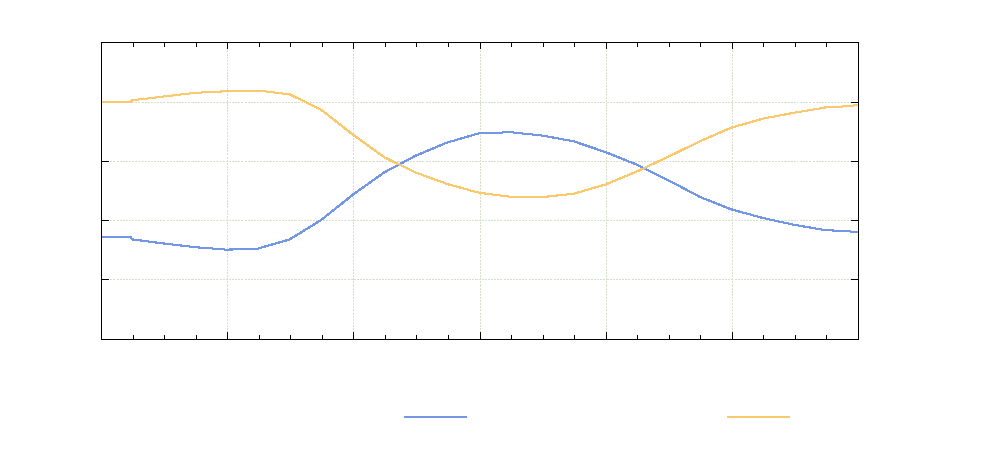
\includegraphics{Graphs/3/Ambient/Ambient}}%
    \gplfronttext
  \end{picture}%
\endgroup
}
			\caption{Average summer ambient air conditions at a South African gold mine.}
			\label{fig: Ambient}
		\end{figure}
		The assumption is made that underground conditions remain constant at each mining level. Pressure and temperature increases with depth as a result of auto compression and rock face temperature. Therefore the conditions can be estimated using only the depth at each level.   
		\subsubsection{Compressors}
		Three compressor models were investigated, each with varying complexity. The models are:
		\begin{itemize}
			\item Air compressor
			\item Dynamic compressor 
			\item Positive displacement compressor
		\end{itemize}  
		The air compressor is a general, simplified model. It requires minimal user inputs by making several assumptions. This is useful when parameters for a compressor are not available. Or when doing a quick preliminary simulation. However, it is not ideal for detailed simulations which require more precision. 
		\par 
		The dynamic compressor components are is more complex, taking into account factors such as heat generated by \gls{polyCof} and inefficiencies within the process. Hence, the model can be used more accurately and for more complex simulations than the general compressor model. However, it should be noted that the dynamic compressor is simplified by several assumptions, for example, a constant efficiency at varying loads. 
		\par 	 
		For most scenarios, the dynamic compressor model is most suitable. This component is modelled by fitting a quadratic curve through three points of operation to obtain an equation for corrected mass flow as a function of the pressure ratio. This characteristic curve of compressor  as shown in figure \ref{fig: Compressor Curve} can be accurately estimated even when only one data point is available by making approximations for the zero flow and pressure points on the curve. Once the flow characteristics of the compressors are set, the efficiency and \gls{polyCof} parameters are calibrated such that the output power and air temperature match the actual or estimated outputs of the compressor.
		
		\begin{figure}[h]
			\centering
			\fbox{% GNUPLOT: LaTeX picture with Postscript
\begingroup
  \makeatletter
  \providecommand\color[2][]{%
    \GenericError{(gnuplot) \space\space\space\@spaces}{%
      Package color not loaded in conjunction with
      terminal option `colourtext'%
    }{See the gnuplot documentation for explanation.%
    }{Either use 'blacktext' in gnuplot or load the package
      color.sty in LaTeX.}%
    \renewcommand\color[2][]{}%
  }%
  \providecommand\includegraphics[2][]{%
    \GenericError{(gnuplot) \space\space\space\@spaces}{%
      Package graphicx or graphics not loaded%
    }{See the gnuplot documentation for explanation.%
    }{The gnuplot epslatex terminal needs graphicx.sty or graphics.sty.}%
    \renewcommand\includegraphics[2][]{}%
  }%
  \providecommand\rotatebox[2]{#2}%
  \@ifundefined{ifGPcolor}{%
    \newif\ifGPcolor
    \GPcolortrue
  }{}%
  \@ifundefined{ifGPblacktext}{%
    \newif\ifGPblacktext
    \GPblacktextfalse
  }{}%
  % define a \g@addto@macro without @ in the name:
  \let\gplgaddtomacro\g@addto@macro
  % define empty templates for all commands taking text:
  \gdef\gplbacktext{}%
  \gdef\gplfronttext{}%
  \makeatother
  \ifGPblacktext
    % no textcolor at all
    \def\colorrgb#1{}%
    \def\colorgray#1{}%
  \else
    % gray or color?
    \ifGPcolor
      \def\colorrgb#1{\color[rgb]{#1}}%
      \def\colorgray#1{\color[gray]{#1}}%
      \expandafter\def\csname LTw\endcsname{\color{white}}%
      \expandafter\def\csname LTb\endcsname{\color{black}}%
      \expandafter\def\csname LTa\endcsname{\color{black}}%
      \expandafter\def\csname LT0\endcsname{\color[rgb]{1,0,0}}%
      \expandafter\def\csname LT1\endcsname{\color[rgb]{0,1,0}}%
      \expandafter\def\csname LT2\endcsname{\color[rgb]{0,0,1}}%
      \expandafter\def\csname LT3\endcsname{\color[rgb]{1,0,1}}%
      \expandafter\def\csname LT4\endcsname{\color[rgb]{0,1,1}}%
      \expandafter\def\csname LT5\endcsname{\color[rgb]{1,1,0}}%
      \expandafter\def\csname LT6\endcsname{\color[rgb]{0,0,0}}%
      \expandafter\def\csname LT7\endcsname{\color[rgb]{1,0.3,0}}%
      \expandafter\def\csname LT8\endcsname{\color[rgb]{0.5,0.5,0.5}}%
    \else
      % gray
      \def\colorrgb#1{\color{black}}%
      \def\colorgray#1{\color[gray]{#1}}%
      \expandafter\def\csname LTw\endcsname{\color{white}}%
      \expandafter\def\csname LTb\endcsname{\color{black}}%
      \expandafter\def\csname LTa\endcsname{\color{black}}%
      \expandafter\def\csname LT0\endcsname{\color{black}}%
      \expandafter\def\csname LT1\endcsname{\color{black}}%
      \expandafter\def\csname LT2\endcsname{\color{black}}%
      \expandafter\def\csname LT3\endcsname{\color{black}}%
      \expandafter\def\csname LT4\endcsname{\color{black}}%
      \expandafter\def\csname LT5\endcsname{\color{black}}%
      \expandafter\def\csname LT6\endcsname{\color{black}}%
      \expandafter\def\csname LT7\endcsname{\color{black}}%
      \expandafter\def\csname LT8\endcsname{\color{black}}%
    \fi
  \fi
    \setlength{\unitlength}{0.0500bp}%
    \ifx\gptboxheight\undefined%
      \newlength{\gptboxheight}%
      \newlength{\gptboxwidth}%
      \newsavebox{\gptboxtext}%
    \fi%
    \setlength{\fboxrule}{0.5pt}%
    \setlength{\fboxsep}{1pt}%
\begin{picture}(9360.00,4032.00)%
    \gplgaddtomacro\gplbacktext{%
      \colorrgb{0.00,0.00,0.00}%
      \put(814,704){\makebox(0,0)[r]{\strut{}$0$}}%
      \colorrgb{0.00,0.00,0.00}%
      \put(814,1261){\makebox(0,0)[r]{\strut{}$100$}}%
      \colorrgb{0.00,0.00,0.00}%
      \put(814,1818){\makebox(0,0)[r]{\strut{}$200$}}%
      \colorrgb{0.00,0.00,0.00}%
      \put(814,2375){\makebox(0,0)[r]{\strut{}$300$}}%
      \colorrgb{0.00,0.00,0.00}%
      \put(814,2932){\makebox(0,0)[r]{\strut{}$400$}}%
      \colorrgb{0.00,0.00,0.00}%
      \put(814,3489){\makebox(0,0)[r]{\strut{}$500$}}%
      \colorrgb{0.00,0.00,0.00}%
      \put(946,484){\makebox(0,0){\strut{}$0$}}%
      \colorrgb{0.00,0.00,0.00}%
      \put(1948,484){\makebox(0,0){\strut{}$2$}}%
      \colorrgb{0.00,0.00,0.00}%
      \put(2950,484){\makebox(0,0){\strut{}$4$}}%
      \colorrgb{0.00,0.00,0.00}%
      \put(3952,484){\makebox(0,0){\strut{}$6$}}%
      \colorrgb{0.00,0.00,0.00}%
      \put(4954,484){\makebox(0,0){\strut{}$8$}}%
      \colorrgb{0.00,0.00,0.00}%
      \put(5956,484){\makebox(0,0){\strut{}$10$}}%
      \colorrgb{0.00,0.00,0.00}%
      \put(6958,484){\makebox(0,0){\strut{}$12$}}%
      \colorrgb{0.00,0.00,0.00}%
      \put(7960,484){\makebox(0,0){\strut{}$14$}}%
      \colorrgb{0.00,0.00,0.00}%
      \put(8962,484){\makebox(0,0){\strut{}$16$}}%
      \csname LTb\endcsname%
      \put(5455,3043){\makebox(0,0)[l]{\strut{}$f(x) = -2.586x^2 + 7.788x + 494$}}%
    }%
    \gplgaddtomacro\gplfronttext{%
      \csname LTb\endcsname%
      \put(176,2235){\rotatebox{-270}{\makebox(0,0){\strut{}Mass flow ($kg^3/s/\sqrt(k)/Bar$)}}}%
      \put(4954,154){\makebox(0,0){\strut{}Pressure ratio}}%
    }%
    \gplbacktext
    \put(0,0){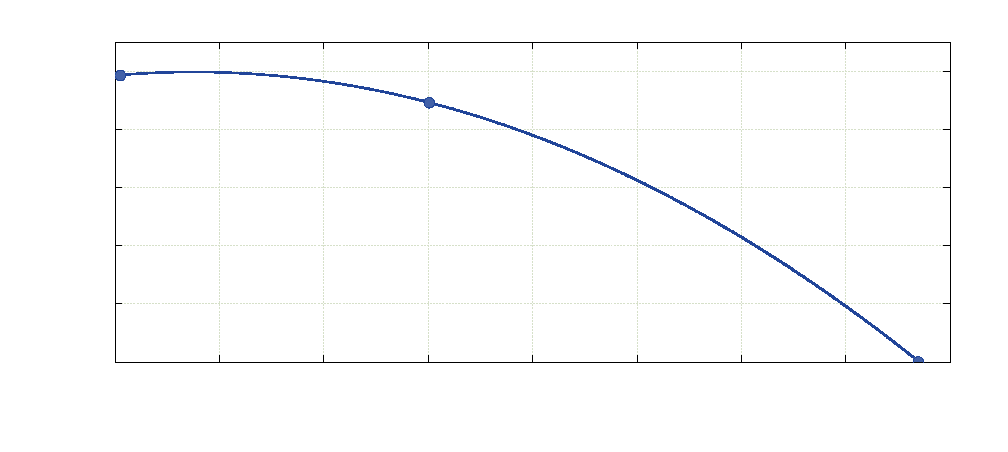
\includegraphics{Graphs/3/AproxCurve/AproxCurve}}%
    \gplfronttext
  \end{picture}%
\endgroup
}
			\caption{Estimating the characteristic curve of a compressor by fitting a quadratic function to points of operation.}
			\label{fig: Compressor Curve}
		\end{figure}

		\par
		Once the models are accurately calibrated, the compressor component is integrated to the air network in the arrangement shown in figure \ref{fig: Compressor models}. The Compressor is connected to the inlet air source via an inlet pipe and air node and to the rest of the network via an air node and outlet pipe. This is is to allow the inlet and outlet parameters and conditions to be be monitored and controlled.
		\begin{figure}[h]
			\centering
			\fbox{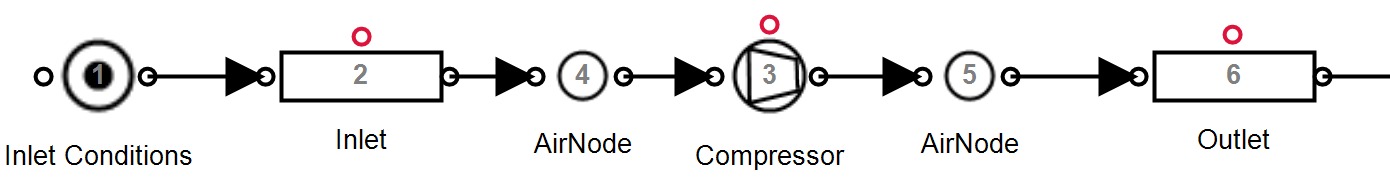
\includegraphics[trim =-4cm 0 -4cm 0cm, width=\textwidth]{Images/3/Compressors}}
			\caption{Integrating the compressor component into the simulation.}
			\label{fig: Compressor models}
		\end{figure}		

		\subsubsection{Demand/leak}
			A flow demand represents any air flow leaving the network. This includes equipment that uses air such as drills and agitators etc. as well as inefficiencies like leaks and open pipes. Generally the air flow is dependent on pressure and the specific resistance to flow of the outlet. 
			\par 
			The resistance of the flow demand can be obtained using the inlet pressure, outlet pressure and flow. If the flow is not known, a reasonably accurate estimation can be made by calculating the expected flow from the size of the outlet. The air demand may vary throughout the day. For example, a mining section may utilise more machines during certain periods of the day. A schedule is used to replicate this in the simulation. Figure \ref{fig: Demand component} shows how a calibrated air demand or leak is integrated into the simulation.
			
			\begin{figure}[h]
				\centering
				\fbox{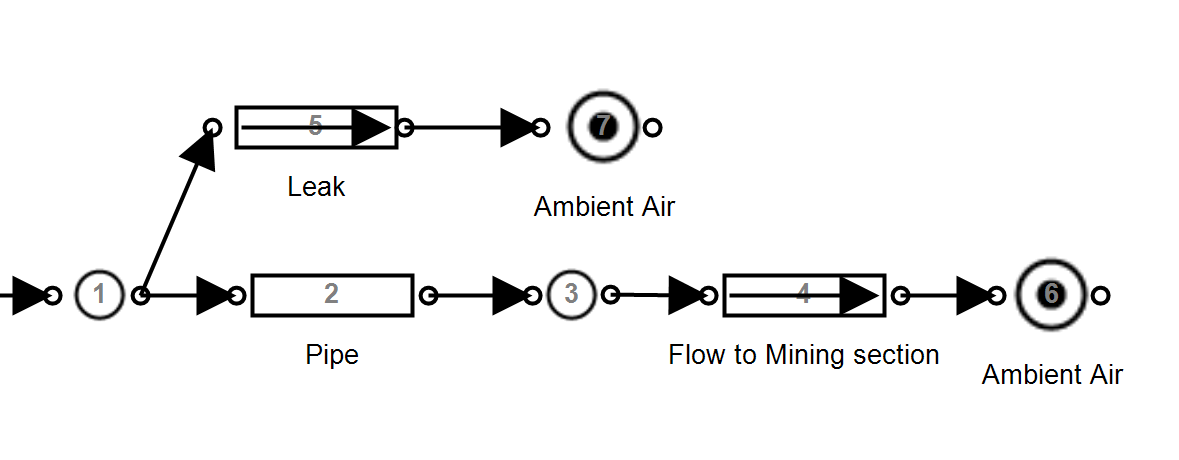
\includegraphics[trim =-12cm 0.5cm -12cm 0.5cmcm, width=\textwidth]{Images/3/AirDemand}}
				\caption{Implementing flow demands and leaks into the simulation.} 
				\label{fig: Demand component}
			\end{figure}
		\subsubsection{Compressed air control}\label{Controllers}
			Simulation components need to be dynamically controlled as in the actual air network. Control is typically implemented on compressors and valves throughout the network to follow certain set-points and schedules. It is important to not only include the controllers in the simulation, but to replicate the non-linearities, limitations and responsiveness related to their use. This ensures the model reacts in the same way the actual network would, improving accuracy.
			\par 
			On a typical mine, compressors power is controlled to ensure that the discharge pressure matches a specified set-point. This control is achieved through either \glspl{vsd} (or \glspl{vfd}) and guide-vain control. \glspl{vfd} provides a wide range of power control and can be estimated using a \gls{pi} controller as in figure \ref{fig: Controller models} where discharge pressure is used as feedback for the controller. 
	\begin{figure}[h]
		\centering
		\fbox{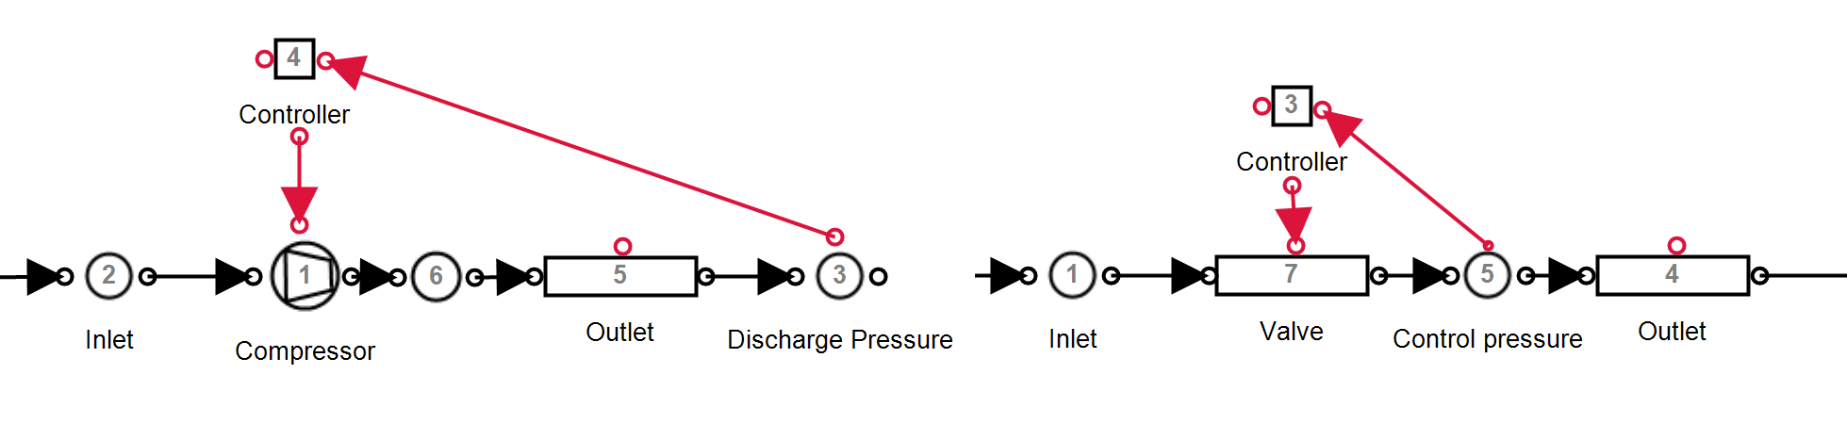
\includegraphics[trim =-4cm 0 -4cm 0cm, width=\textwidth]{Images/3/Controller}}
		\caption{Control components in \gls{stb}.}
		\label{fig: Controller models}
	\end{figure}
		Guide vains are most commonly used in mining to control compressors. This entails controlling the position of the inlet guide vain . The guide vain is opened or closed to control the compressors discharge pressure.  Manipulating the guide vain position will affect the power the compressor inputs into the system. Figure \ref{fig: Guide vain position} shows the relationship between  power and guide vain position. This can be approximated as a linearly where A guide vain position of 40\%  retales to an output power of about 60\% of the maximum power. When more pressure is required than can be obtained with the guide vains fully opened, another compressor is needed to operate. 
		\begin{figure}[h]
			\centering
			\fbox{% GNUPLOT: LaTeX picture with Postscript
\begingroup
  \makeatletter
  \providecommand\color[2][]{%
    \GenericError{(gnuplot) \space\space\space\@spaces}{%
      Package color not loaded in conjunction with
      terminal option `colourtext'%
    }{See the gnuplot documentation for explanation.%
    }{Either use 'blacktext' in gnuplot or load the package
      color.sty in LaTeX.}%
    \renewcommand\color[2][]{}%
  }%
  \providecommand\includegraphics[2][]{%
    \GenericError{(gnuplot) \space\space\space\@spaces}{%
      Package graphicx or graphics not loaded%
    }{See the gnuplot documentation for explanation.%
    }{The gnuplot epslatex terminal needs graphicx.sty or graphics.sty.}%
    \renewcommand\includegraphics[2][]{}%
  }%
  \providecommand\rotatebox[2]{#2}%
  \@ifundefined{ifGPcolor}{%
    \newif\ifGPcolor
    \GPcolortrue
  }{}%
  \@ifundefined{ifGPblacktext}{%
    \newif\ifGPblacktext
    \GPblacktextfalse
  }{}%
  % define a \g@addto@macro without @ in the name:
  \let\gplgaddtomacro\g@addto@macro
  % define empty templates for all commands taking text:
  \gdef\gplbacktext{}%
  \gdef\gplfronttext{}%
  \makeatother
  \ifGPblacktext
    % no textcolor at all
    \def\colorrgb#1{}%
    \def\colorgray#1{}%
  \else
    % gray or color?
    \ifGPcolor
      \def\colorrgb#1{\color[rgb]{#1}}%
      \def\colorgray#1{\color[gray]{#1}}%
      \expandafter\def\csname LTw\endcsname{\color{white}}%
      \expandafter\def\csname LTb\endcsname{\color{black}}%
      \expandafter\def\csname LTa\endcsname{\color{black}}%
      \expandafter\def\csname LT0\endcsname{\color[rgb]{1,0,0}}%
      \expandafter\def\csname LT1\endcsname{\color[rgb]{0,1,0}}%
      \expandafter\def\csname LT2\endcsname{\color[rgb]{0,0,1}}%
      \expandafter\def\csname LT3\endcsname{\color[rgb]{1,0,1}}%
      \expandafter\def\csname LT4\endcsname{\color[rgb]{0,1,1}}%
      \expandafter\def\csname LT5\endcsname{\color[rgb]{1,1,0}}%
      \expandafter\def\csname LT6\endcsname{\color[rgb]{0,0,0}}%
      \expandafter\def\csname LT7\endcsname{\color[rgb]{1,0.3,0}}%
      \expandafter\def\csname LT8\endcsname{\color[rgb]{0.5,0.5,0.5}}%
    \else
      % gray
      \def\colorrgb#1{\color{black}}%
      \def\colorgray#1{\color[gray]{#1}}%
      \expandafter\def\csname LTw\endcsname{\color{white}}%
      \expandafter\def\csname LTb\endcsname{\color{black}}%
      \expandafter\def\csname LTa\endcsname{\color{black}}%
      \expandafter\def\csname LT0\endcsname{\color{black}}%
      \expandafter\def\csname LT1\endcsname{\color{black}}%
      \expandafter\def\csname LT2\endcsname{\color{black}}%
      \expandafter\def\csname LT3\endcsname{\color{black}}%
      \expandafter\def\csname LT4\endcsname{\color{black}}%
      \expandafter\def\csname LT5\endcsname{\color{black}}%
      \expandafter\def\csname LT6\endcsname{\color{black}}%
      \expandafter\def\csname LT7\endcsname{\color{black}}%
      \expandafter\def\csname LT8\endcsname{\color{black}}%
    \fi
  \fi
    \setlength{\unitlength}{0.0500bp}%
    \ifx\gptboxheight\undefined%
      \newlength{\gptboxheight}%
      \newlength{\gptboxwidth}%
      \newsavebox{\gptboxtext}%
    \fi%
    \setlength{\fboxrule}{0.5pt}%
    \setlength{\fboxsep}{1pt}%
\begin{picture}(9360.00,4032.00)%
    \gplgaddtomacro\gplbacktext{%
      \colorrgb{0.00,0.00,0.00}%
      \put(814,704){\makebox(0,0)[r]{\strut{}$0$}}%
      \colorrgb{0.00,0.00,0.00}%
      \put(814,1214){\makebox(0,0)[r]{\strut{}$20$}}%
      \colorrgb{0.00,0.00,0.00}%
      \put(814,1725){\makebox(0,0)[r]{\strut{}$40$}}%
      \colorrgb{0.00,0.00,0.00}%
      \put(814,2235){\makebox(0,0)[r]{\strut{}$60$}}%
      \colorrgb{0.00,0.00,0.00}%
      \put(814,2746){\makebox(0,0)[r]{\strut{}$80$}}%
      \colorrgb{0.00,0.00,0.00}%
      \put(814,3256){\makebox(0,0)[r]{\strut{}$100$}}%
      \colorrgb{0.00,0.00,0.00}%
      \put(814,3767){\makebox(0,0)[r]{\strut{}$120$}}%
      \colorrgb{0.00,0.00,0.00}%
      \put(946,484){\makebox(0,0){\strut{}$0$}}%
      \colorrgb{0.00,0.00,0.00}%
      \put(2282,484){\makebox(0,0){\strut{}$20$}}%
      \colorrgb{0.00,0.00,0.00}%
      \put(3618,484){\makebox(0,0){\strut{}$40$}}%
      \colorrgb{0.00,0.00,0.00}%
      \put(4954,484){\makebox(0,0){\strut{}$60$}}%
      \colorrgb{0.00,0.00,0.00}%
      \put(6290,484){\makebox(0,0){\strut{}$80$}}%
      \colorrgb{0.00,0.00,0.00}%
      \put(7626,484){\makebox(0,0){\strut{}$100$}}%
      \colorrgb{0.00,0.00,0.00}%
      \put(8962,484){\makebox(0,0){\strut{}$120$}}%
    }%
    \gplgaddtomacro\gplfronttext{%
      \csname LTb\endcsname%
      \put(176,2235){\rotatebox{-270}{\makebox(0,0){\strut{}Output power (\%)}}}%
      \put(4954,154){\makebox(0,0){\strut{}Guide Vain Position (\%)}}%
    }%
    \gplbacktext
    \put(0,0){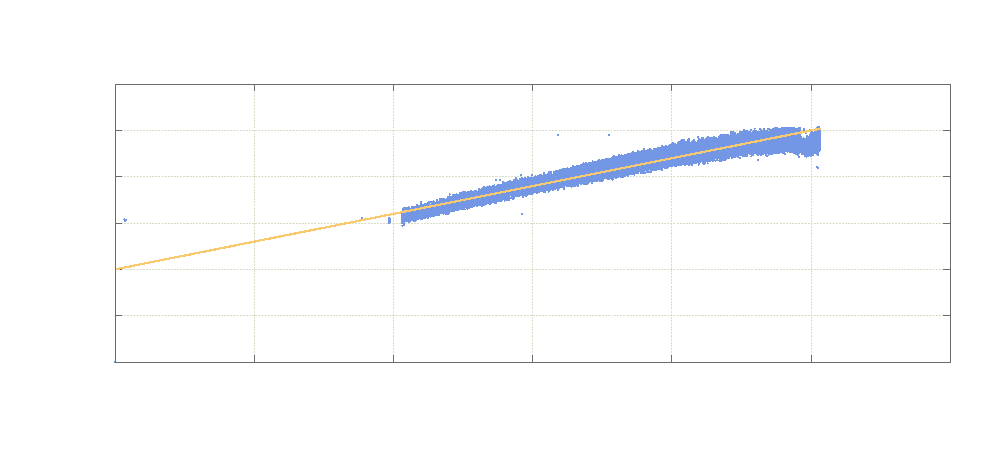
\includegraphics{Graphs/1/GuideVainPosition/GuideVainPosition}}%
    \gplfronttext
  \end{picture}%
\endgroup
}
			\caption[The relation between guide vain position and compressor output power.]{The relation between guide vain position and compressor output power.}
			\label{fig: Guide vain position}
		\end{figure}
		\par
		A guide vain controller is modelled using a \gls{pi} controller component. However, the limitations of guide vain control, as represented in figure \ref{fig: Guide vain position}, must be implemented in the controller. This is done by using a minimum output that would match the minimum power reduction the guide vain achieved by closing the guide vain. For example, a \gls{pi} controller for the compressor from figure \ref{fig: Guide vain position} would have a minimum control output of approximately 60\%.
		\par 
		Mines utilize control valves at underground sections to control the pressure at individual mining stations independently \cite{Heyns2014Masters}. Controlling of valve components is performed similarly as control of the compressor components. As shown in figure \ref{fig: Controller models} the outlet pressure is used as feedback for a pi controller. The controller output is mapped to the valve fraction of a pipe component.
		\begin{figure}[h]
			\centering
			\fbox{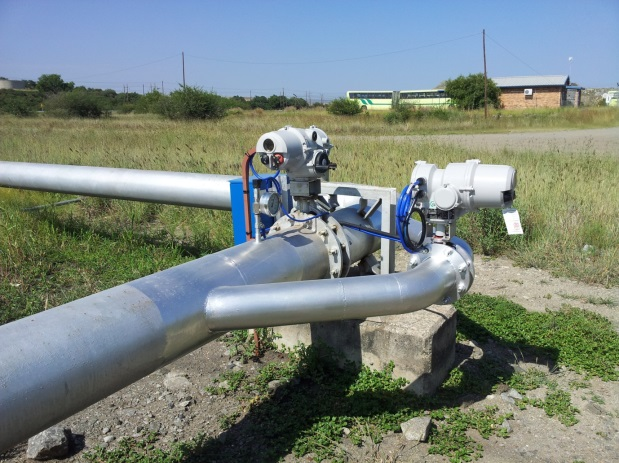
\includegraphics[trim =-2cm 0 -2cm 0cm, width=\textwidth]{Images/3/Valve.jpg}}
			\caption[An example of a compressed air control valve.]{An example of a compressed air control valve\cite{van2015implementation}.} 
			\label{fig: Control}
		\end{figure}
		\subsubsection{Compressed air after-cooling}
		The air compression process generates significant heat. Compressed air at high temperatures contains a large amount of water vapour. To prevent condensation later in the air network, improve the system capacity and protect equipment from excessive heat, after-coolers are installed to the outlet of the compressor \cite{schroeder2009energy}.
		\par 
		After-cooling reduces the compressed air temperature to within a margin of ambient. This cooling could have a large effect on the performance of the network. Hence, including after-cooling to the simulation model should improve accuracy.
		\par 
		To replicate this effect, a heat transfer node can be added to the outlet of the compressor component. \gls{stb} Utilizes the following heat transfer parameters of the air node to solve for outlet temperature: 
		\begin{tabular}{p{1.3cm}p{13cm}}
			$Area$ & The heat transfer area ($m^2$) \\
			$UA$ & Heat transfer coefficient ($kW/^{\circ} C$) \\
			$T_{amb}$ & Ambient air temperature ($^{\circ} C$) \\
		\end{tabular} \\	
	\subsection{Verification of simulation model}
		- Steps to validate  the model accuracy - Compare parameters to actuals\\
		- First principles     - Comparison to other models
	\subsection{Simulation inputs}
		The inputs of a simulation are any parameters that do not remain static, or follow the same profile in day to day operation of the system. Examples of such parameters in a compressed air simulation are:
		\begin{itemize}
			\item Simulation period
			\item Surface ambient conditions
			\item Machine operation schedules
			\item Air demands
			\item Operational changes
		\end{itemize} 
		Changing the simulation baseline period for a calibrated simulation should only require the updating of the input parameters. Figured \ref{fig: Compressor schedule} shows an example of a changing compressor schedule where an input parameter would need to be updated in the simulation.
		\begin{figure}[h]
			\centering
			\fbox{% GNUPLOT: LaTeX picture with Postscript
\begingroup
  \makeatletter
  \providecommand\color[2][]{%
    \GenericError{(gnuplot) \space\space\space\@spaces}{%
      Package color not loaded in conjunction with
      terminal option `colourtext'%
    }{See the gnuplot documentation for explanation.%
    }{Either use 'blacktext' in gnuplot or load the package
      color.sty in LaTeX.}%
    \renewcommand\color[2][]{}%
  }%
  \providecommand\includegraphics[2][]{%
    \GenericError{(gnuplot) \space\space\space\@spaces}{%
      Package graphicx or graphics not loaded%
    }{See the gnuplot documentation for explanation.%
    }{The gnuplot epslatex terminal needs graphicx.sty or graphics.sty.}%
    \renewcommand\includegraphics[2][]{}%
  }%
  \providecommand\rotatebox[2]{#2}%
  \@ifundefined{ifGPcolor}{%
    \newif\ifGPcolor
    \GPcolortrue
  }{}%
  \@ifundefined{ifGPblacktext}{%
    \newif\ifGPblacktext
    \GPblacktextfalse
  }{}%
  % define a \g@addto@macro without @ in the name:
  \let\gplgaddtomacro\g@addto@macro
  % define empty templates for all commands taking text:
  \gdef\gplbacktext{}%
  \gdef\gplfronttext{}%
  \makeatother
  \ifGPblacktext
    % no textcolor at all
    \def\colorrgb#1{}%
    \def\colorgray#1{}%
  \else
    % gray or color?
    \ifGPcolor
      \def\colorrgb#1{\color[rgb]{#1}}%
      \def\colorgray#1{\color[gray]{#1}}%
      \expandafter\def\csname LTw\endcsname{\color{white}}%
      \expandafter\def\csname LTb\endcsname{\color{black}}%
      \expandafter\def\csname LTa\endcsname{\color{black}}%
      \expandafter\def\csname LT0\endcsname{\color[rgb]{1,0,0}}%
      \expandafter\def\csname LT1\endcsname{\color[rgb]{0,1,0}}%
      \expandafter\def\csname LT2\endcsname{\color[rgb]{0,0,1}}%
      \expandafter\def\csname LT3\endcsname{\color[rgb]{1,0,1}}%
      \expandafter\def\csname LT4\endcsname{\color[rgb]{0,1,1}}%
      \expandafter\def\csname LT5\endcsname{\color[rgb]{1,1,0}}%
      \expandafter\def\csname LT6\endcsname{\color[rgb]{0,0,0}}%
      \expandafter\def\csname LT7\endcsname{\color[rgb]{1,0.3,0}}%
      \expandafter\def\csname LT8\endcsname{\color[rgb]{0.5,0.5,0.5}}%
    \else
      % gray
      \def\colorrgb#1{\color{black}}%
      \def\colorgray#1{\color[gray]{#1}}%
      \expandafter\def\csname LTw\endcsname{\color{white}}%
      \expandafter\def\csname LTb\endcsname{\color{black}}%
      \expandafter\def\csname LTa\endcsname{\color{black}}%
      \expandafter\def\csname LT0\endcsname{\color{black}}%
      \expandafter\def\csname LT1\endcsname{\color{black}}%
      \expandafter\def\csname LT2\endcsname{\color{black}}%
      \expandafter\def\csname LT3\endcsname{\color{black}}%
      \expandafter\def\csname LT4\endcsname{\color{black}}%
      \expandafter\def\csname LT5\endcsname{\color{black}}%
      \expandafter\def\csname LT6\endcsname{\color{black}}%
      \expandafter\def\csname LT7\endcsname{\color{black}}%
      \expandafter\def\csname LT8\endcsname{\color{black}}%
    \fi
  \fi
    \setlength{\unitlength}{0.0500bp}%
    \ifx\gptboxheight\undefined%
      \newlength{\gptboxheight}%
      \newlength{\gptboxwidth}%
      \newsavebox{\gptboxtext}%
    \fi%
    \setlength{\fboxrule}{0.5pt}%
    \setlength{\fboxsep}{1pt}%
\begin{picture}(9360.00,4032.00)%
    \gplgaddtomacro\gplbacktext{%
      \colorrgb{0.00,0.00,0.00}%
      \put(550,924){\makebox(0,0)[r]{\strut{}}}%
      \colorrgb{0.00,0.00,0.00}%
      \put(550,1258){\makebox(0,0)[r]{\strut{}$1$}}%
      \colorrgb{0.00,0.00,0.00}%
      \put(550,1593){\makebox(0,0)[r]{\strut{}$2$}}%
      \colorrgb{0.00,0.00,0.00}%
      \put(550,1927){\makebox(0,0)[r]{\strut{}$3$}}%
      \colorrgb{0.00,0.00,0.00}%
      \put(550,2262){\makebox(0,0)[r]{\strut{}$4$}}%
      \colorrgb{0.00,0.00,0.00}%
      \put(550,2596){\makebox(0,0)[r]{\strut{}$5$}}%
      \colorrgb{0.00,0.00,0.00}%
      \put(550,2931){\makebox(0,0)[r]{\strut{}$6$}}%
      \colorrgb{0.00,0.00,0.00}%
      \put(550,3265){\makebox(0,0)[r]{\strut{}$7$}}%
      \colorrgb{0.00,0.00,0.00}%
      \put(550,3600){\makebox(0,0)[r]{\strut{}$8$}}%
      \colorrgb{0.00,0.00,0.00}%
      \put(682,704){\makebox(0,0){\strut{}00:00}}%
      \colorrgb{0.00,0.00,0.00}%
      \put(2062,704){\makebox(0,0){\strut{}04:00}}%
      \colorrgb{0.00,0.00,0.00}%
      \put(3442,704){\makebox(0,0){\strut{}08:00}}%
      \colorrgb{0.00,0.00,0.00}%
      \put(4822,704){\makebox(0,0){\strut{}12:00}}%
      \colorrgb{0.00,0.00,0.00}%
      \put(6202,704){\makebox(0,0){\strut{}16:00}}%
      \colorrgb{0.00,0.00,0.00}%
      \put(7582,704){\makebox(0,0){\strut{}20:00}}%
      \colorrgb{0.00,0.00,0.00}%
      \put(8962,704){\makebox(0,0){\strut{}00:00}}%
    }%
    \gplgaddtomacro\gplfronttext{%
      \csname LTb\endcsname%
      \put(176,2345){\rotatebox{-270}{\makebox(0,0){\strut{}Compressor}}}%
      \put(4822,374){\makebox(0,0){\strut{}Time of Day}}%
      \csname LTb\endcsname%
      \put(3967,100){\makebox(0,0)[r]{\strut{}Period 1}}%
      \csname LTb\endcsname%
      \put(5878,100){\makebox(0,0)[r]{\strut{}Period 2}}%
    }%
    \gplbacktext
    \put(0,0){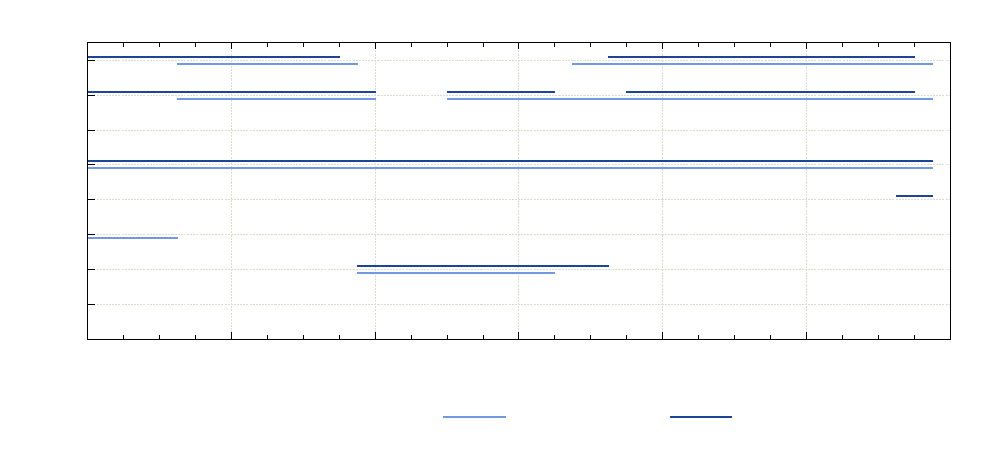
\includegraphics{Graphs/3/CompSelection/CompSelection}}%
    \gplfronttext
  \end{picture}%
\endgroup
}
			\caption{An example of two baseline periods, showing a changed compressor schedule.}
			\label{fig: Compressor schedule}
		\end{figure}
	\subsection{Summary}
	\textit{Unfinished}
\newpage
\section{Implementation of simulation method}
	\subsection{Preamble}
		Once a simulation has been developed and verified, the implementation of interventions and scenarios follows. In this section, the approach of implementation the simulation methodology, and analysis of interventions will be discussed.
	\subsection{Analyses of data}
		- Baseline vs Optimised analysis \\
		- identification of further improvements\\
		\textit{Unfinished}
	\subsection{Quantifying operational improvements}
		- Estimating cost savings \\
		- Reporting feedback to the mine\\
		\textit{Unfinished}
	\subsection{Summary}
\section{Conclusion}

%Chapter 4
\chapter{Results and validation}
%\pagenumbering{gobble}
\vspace{38em}

\hrulefill
\\
\enquote*{\textit{Quote.}} - Somebody\\
\newpage
\section{Preamble}
\section{Case study: Mine A \color{blue}(Kusasalethu)}
	\subsection{Background}
	\subsection{Scenario 1. Refuge bay simulation}
	tested scenario where all excessive leaking valves are removed.
	refuge bays savings 1MW E.E.
	\subsection{Scenario 2. Closing off levels/stopes}
	
	\subsection{Scenario 3. Periodic simulation}
	\subsection{Summary}
\section{Case study: Mine B \color{blue}(Beatrix 123)}
	\subsection{Background}
	\subsection{Compressor set points}
	\subsection{Control valves set points}
	\subsection{Summary}
\section{Validation of results}
\section{Conclusion}
%Chapter 5
\chapter{Conclusion}
\thispagestyle{empty}
\vspace{40em}
\hrulefill
\\
%\enquote*{\textit{Quote.}} - Somebody\\
\newpage
		\section{Preamble}
		Chapter 5 serves as the conclusion of this dissertation and it provides an overview of the complete dissertation. This overview summarises the work done in the preceding chapters and discusses the limitations of the study as well as recommendations for future work to be done in the field.
	 \section{Dissertation overview}
		The South African mining sector is currently facing significant challenges that pose a risk to the profitability of the industry. A central challenge that faces the industry is that of rising operational costs. Energy costs constitute a significant portion of the cost increases as energy tariff increases have consistently exceeded inflation over the past ten years.
	 \par
		Compressed air systems do not only consume the largest portion of energy used in a mine, but they were also shown to be largely inefficient. It is therefore reasoned that the greatest energy impact can be achieved through interventions in respect of compressed air networks.
	 \par 
		Energy interventions in mining compressed air systems have been performed in the past. However, compressed air simulation has not been used to its full potential. The specific effects of interventions imply minimal risk, by using new computer modelling and simulation tools for compressed air systems. This will lead to further energy and cost reductions as well as other potential improvements in the operation of a mine.
	 \par 
	 A review of background and literature was performed. The purpose of the review was to provide background on mining compressed air networks and to evaluate literature pertaining to compressed air energy interventions, as well as to simulation usage in the mining industry in general and compressed air systems in particular.
	 \par 
		A methodology was developed for compressed air simulation, using the findings that emerged from the literature review. The method describes the simulation procedure in three steps, namely: investigate the system; develop a simulation model; and execute the simulation scenarios.
	 \par 
The simulation methodology was implemented with case studies that were performed on the compressed air systems of two different mines. A full system investigation was conducted in each study. From the data and information obtained from the investigation, simulation models were developed for both systems. The models were verified using measurement data from the physical system and they were used to simulate various operational scenarios.
	 \par 
In Case Study 1, two scenarios were simulated. The results of the first scenario – reducing compressor  set-points – showed a potential power reduction of 0.46 $MW$ PC, which would result in a yearly energy cost saving of R0.37m. Scenario 2 – reducing underground control valve pressure – showed a potential power reduction of 1.0 $MW$ PC, which would result in a yearly energy cost saving of R0.91m. The result of the simulation was validated by comparing it with the actual results of the test conducted on the physical system.
	 \par
	 In Case Study 2, two scenarios were simulated. The first scenario looked at reducing refuge bay leaks. The results showed a potential energy efficiency improvement of 0.92 $MW$, which would result in an annual energy cost saving of R5.17m. A further pressure improvement of 15 $kPa$ during the drilling time was identified. In Scenario 2, optimising peak-time demand through station and in-stope control was investigated. The results showed that a potential power reduction of up to 2.0 $MW$ \gls{pc} could be obtained. This optimisation would lead to energy cost saving of R0.91m per year.
	 \par 
	 In Case Study 3, repeated periodic simulations were analysed. The investigation aimed to check the validity of simulation models and to identify when major shifts in a compressed air system’s operation occur. A faulty power meter was identified. However, based on the pressure and flow process parameters, the analysis showed that the model accurately represented the system over the period of repeated simulations.
	 \par
	 Implementing the simulation methodology developed in this study in other gold and PGM mines' compressed air systems would  bring about significant energy cost savings and operational improvements for the industry. It was estimated that up to a 30 $MW$ energy efficiency improvement could be achieved. This increase in efficiency would lead to cost savings of up to R240m per year for the industry. 
	 %\section{Limits of this study}
	 \section{Recommendations for future studies}
	 This study focused on operational improvements in compressed air systems as they offered the largest scope for energy improvement. However, an integrated simulation approach could also lead to significant operational improvements in other large industrial systems, such as ventilation and water reticulation.
	 \par
	 \clearpage
	 Simulation model details, are dependent on system boundary selection as well as varying air properties. Since the current study did not investigate the actual effect of different boundary selections or differing input conditions with regard to simulation accuracy, there is scope for a sensitivity analysis to analyse the accuracy of simulations with different boundary choices.
	 \par
	 A major limiting factor in integrated simulations of large systems is the availability of reliable data. A study that focuses on the value of instrumentation for simulation and system improvement identification is recommended. The study should investigate the availability of data in mining systems and the  relation with energy operational improvement measures.
	 \par 
	 In Case Study 2, an additional pressure benefit was identified in one of the simulated scenarios. It is recommended that future studies investigate the financial impact of pressure improvements that may result from quicker/more efficient drilling. Finally, a future study should be performed to validate the simulation results achieved in Case Study 2. This can be achieved through practical tests executed on the physical system.

\bibliographystyle{IEEEtran}
\addcontentsline{toc}{chapter}{Bibliography}
\bibliography{Bibliography}
%Appendices
\begin{appendices}
\chapter{1}
\chapter{2}
\end{appendices}

\glsaddall
\end{document}